\documentclass[tikz,10pt]{standalone}

%%%%%%%%%%%%%%%%%%%%%%%%%%%%%%%%%%%%%%%%%
%                                       %
%                MY COLORS              %
%                                       %
%%%%%%%%%%%%%%%%%%%%%%%%%%%%%%%%%%%%%%%%%
 \definecolor{ccred}{cmyk}{0, 0.87, 0.8, 0.21}
 \definecolor{ccargile}{RGB}{239,239,239}
 %%%%%%%%%%%%%%%%%%%%%%%%%%%%%%%%%%%%%%%%%

\begin{document}
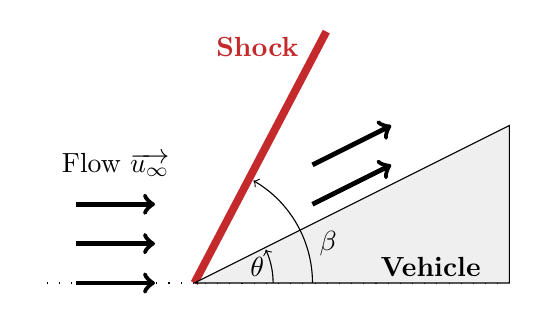
\begin{tikzpicture}[scale=1]
 
  % Axis
  \draw (-2,0) node (begin) {};
  \draw (4,0) node (end) {};
  \draw[loosely dotted] (begin) -- (end) ;

  % Oblique schock
  \draw[line width=1mm, ccred, rotate=6] (0,0) -- (2,3);
  \draw(0.8,3.0) node[ccred] (choc) {\textbf{Shock}};

  % Vehicle
  \filldraw[black, fill=ccargile] (0,0) -- (4,0) -- (4,2) -- (0,0) ;
  \draw(3,0.2) node[scale=1] (objet) {\textbf{Vehicle}};
  \draw[->] (1,0) arc (0:25:1cm);
  \draw (0.8,0.2) node {$\theta$};
  
  \draw[->] (1.5,0) arc (0:60:1.5cm);
  \draw (1.7,0.5) node {$\beta$};

  % Flow u vectors
  \draw[->, line width=0.6mm] (-1.5,0) -- (-0.5,0);
  \draw[->, line width=0.6mm] (-1.5,0.5) -- (-0.5,0.5);
  \draw[->, line width=0.6mm] (-1.5,1) -- (-0.5,1);
  \draw(-1,1.5) node[black] (flow) {Flow $\overrightarrow{u_\infty}$};
  
  \draw[->, line width=0.6mm] (1.5,1.5) -- (2.5,2);
  \draw[->, line width=0.6mm] (1.5,1) -- (2.5,1.5);
 

\end{tikzpicture}
\end{document}
